% PART VII — PHASE 18 FUTURE RESEARCH [UNIMPLEMENTED]
\chapter{Chapter 10: Future Scope — Multi-Agent Cooperative Manipulation Architecture}
\section{10.1 Explicit Future-Scope Disclaimer}
CRITICAL PROVENANCE NOTICE: Phase 18 has NOT been implemented, simulated, or verified in this repository. Every architecture and methodology detailed in Chapter 10 constitutes a forward research roadmap building upon the verified Phase 1–17 single-arm baseline.

\section{10.2 Multi-Robot Cooperative Manipulation, MARL, Task Allocation \& Human-Robot Teaming}
A. Multi-Robot Simulation \& Cooperative Manipulation: Extending single-arm cells into dual-Panda tabletop bays requires synchronized contact constraints inside PyBullet/MuJoCo so two manipulators can jointly lift oversized rigid payloads or perform mid-air bimanual re-orientation without inter-arm self-collision.
B. Multi-Agent Reinforcement Learning (MARL) \& CTDE: Centralized Training with Decentralized Execution (Figure 10.1) resolves non-stationarity by feeding global joint states and both action vectors into centralized mixing critics Q\_tot(s\_all, a\_A, a\_B) while executing decentralized local policies pi\_A(a\_A|o\_A) and pi\_B(a\_B|o\_B) at runtime.
C. Distributed Task Allocation, Cooperative Assembly \& Inter-Robot Communication: Combinatorial auctions or Graph Neural Network allocators partition multi-object sorting sequences dynamically between arms, exchanging latent intent embeddings m\_t to prevent workspace deadlocks during shared peg-in-hole handovers.
D. Human-Robot Collaboration, Swarm Intelligence \& Multi-Agent Robustness: Safe velocity separation scaling (ISO/TS 15066 principles), intent-aware trajectory replanning around moving human operators, and robustness under packet-loss delays across multi-agent links remain open theoretical and experimental challenges. Proposed evaluation metrics include joint bimanual grasp success rate, collision-free cycle time, communication bandwidth overhead, and degraded performance when one agent experiences injected sensor latency.

\begin{figure}[htbp]\centering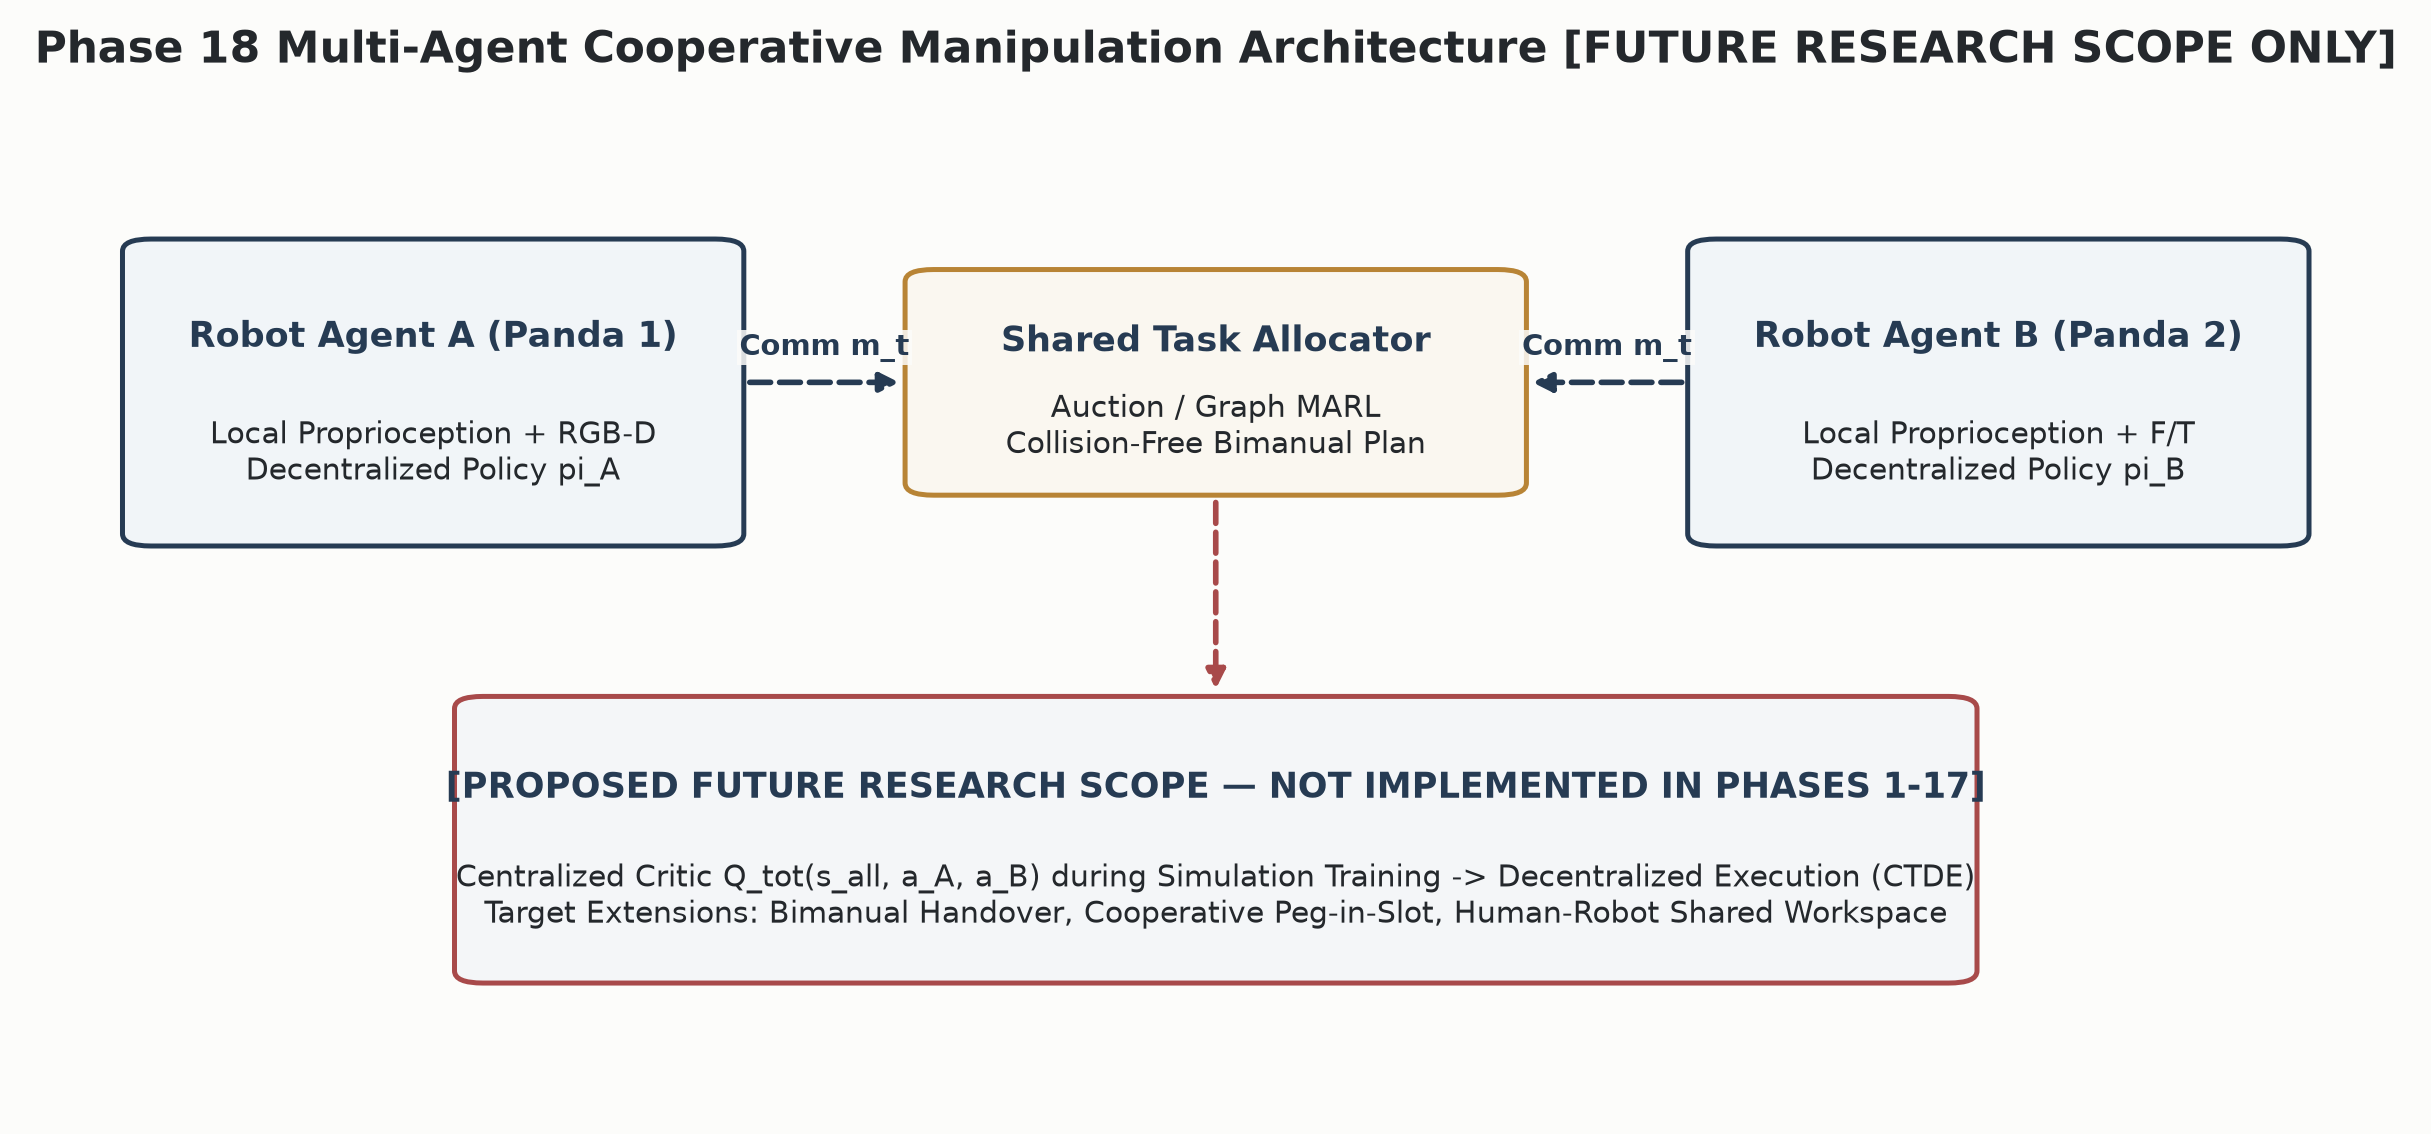
\includegraphics[width=0.9\linewidth]{../../assets/diagrams/diag_13_phase18_multiagent_future.png}\caption{Figure 10.1: Proposed Phase 18 Centralized Training / Decentralized Execution (CTDE) Multi-Agent Cooperative Manipulation architecture [UNIMPLEMENTED].}\end{figure}
\begin{figure}[htbp]\centering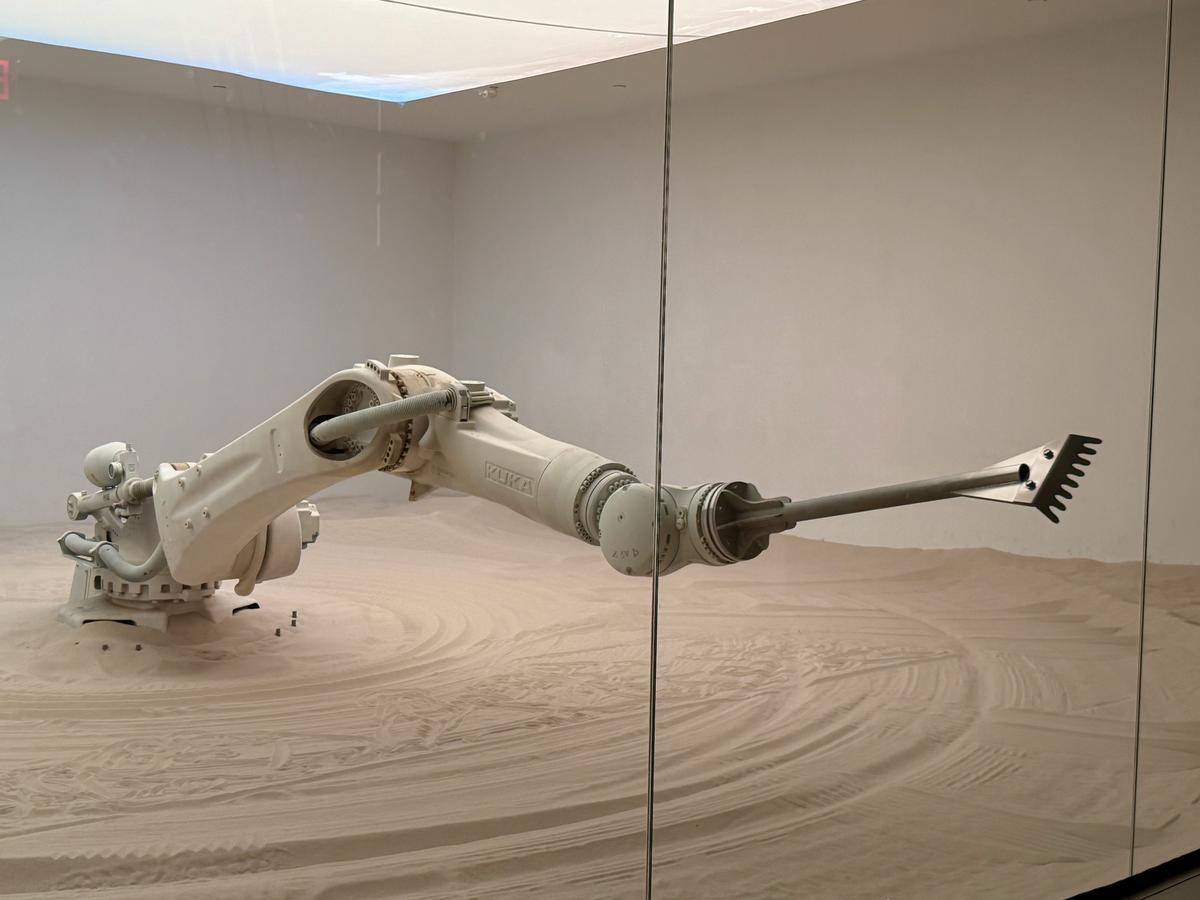
\includegraphics[width=0.9\linewidth]{../../assets/photographs/photo_02_industrial_robot_arm.jpg}\caption{Figure 10.2: Multi-axis industrial serial manipulator illustrating industrial automation hardware scale beyond single tabletop simulation. Source: Wikimedia Commons (KUKA industrial robotic arm performing The Beach - 03.jpg), Author: Oleg Yunakov, License: CC BY-SA 4.0.}\end{figure}